\section{Orderings in sparse Gaussian elimination}
\label{sec:OrderingInSparse}

\subsection{Orderings}
\label{sec:orderings}

\begin{exm}
  \label{exm:reordering}
  Consider the matrix that has the pattern illustrated on the right of
  Figure \ref{fig:ReorderingSparse} with diagonal entries $1.0$ and
  off-diagonal entries $1.1$. The partial pivoting strategy would
  destroy all sparsity because none of the diagonal entries would be
  available as a pivot. However, if we adapt the threshold pivoting
  strategy with $u=0.1$ to the sparse case,  all the
  diagonal entries except the last are available as pivots and the
  sparsity is well preserved.

  \begin{figure}[H]
    \centering
    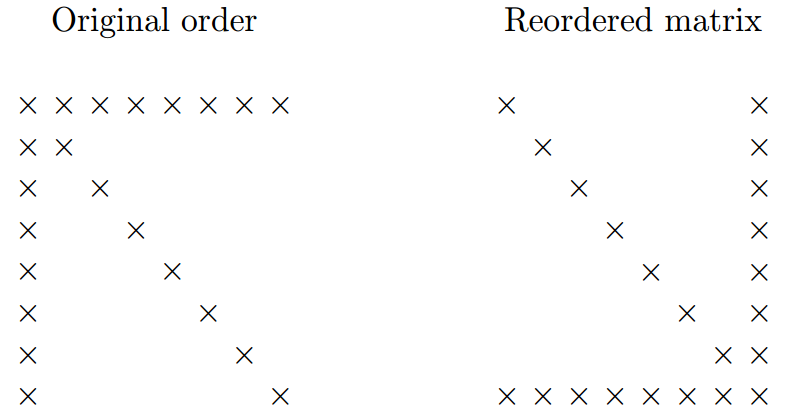
\includegraphics[width=7cm]{png/ReorderingSparse.png}
    \caption{Reordering can preserve sparsity in factorization.}
    \label{fig:ReorderingSparse}
  \end{figure}
\end{exm}

\begin{rmk}
  Ordering the rows and columns to preserve sparsity in Gaussian
  elimination was demonstrated to be effective in the Example
  \ref{exm:reordering}.
  There are four quite different strategies for ordering a sparse
  matrix which are introduced in the following section:
  \begin{enumerate}
  \item We may be able to reorder the matrix to block
    triangular form. We discuss this in Section \ref{sec:GEforSM}. If
    such an ordering exists, we can confine the factorization steps to
    smaller blocks on the diagonal, rather than to the whole matrix.
  \item We consider local strategies where, at each stage of
    the factorization, we choose as pivot the entry that preserves
    sparsity "as well as possible" according to some criteria, which
    will be introduced in Section \ref{sec:LocalPivotal}.
  \item There are methods of preserving sparsity by confining
    fill-ins to particular areas of the matirx, which will be
    developed in Section \ref{sec:BandSolution}.
  \item A strategy under the heading of dissection methods
    looks at the matrix in its entirety, seeking to split the overall
    problem into independent subproblems, which is particularly
    applicable for parallel computing environments. We will discuss in
    Section \ref{sec:Dissection}.
  \end{enumerate}

  There is no single "best" method for preserving sparsity. The
  criteria for what is best is more difficult than it might seem at
  first. For example, the criterion of "least fill-in" might seem to
  be best, but may require a great deal more data structure
  manipulation. 
\end{rmk}
\subsection{Reduction to block triangular form}
\label{sec:GEforSM}
 
\begin{defn}
  \label{defn:BLTF}
  A pattern is worthwhile to seek is the \emph{block lower triangular form}
  \begin{equation}
    \label{eq:BLTF}
    \mathbf{PAQ}=\left[
    \begin{array}{ccccc}
      \mathbf{B}_{11}& & & & \\
     \mathbf{ B}_{21} & \mathbf{B}_{22} & & & \\
      \mathbf{B}_{31} & \mathbf{B}_{32} &\mathbf{B}_{33} & & \\
      \vdots&\vdots&\vdots&\ddots& \\
      \mathbf{B}_{N1}& \mathbf{B}_{N2}& \mathbf{B}_{N3} & \cdots& \mathbf{B}_{NN}\\
    \end{array}
  \right]
  \end{equation}
\end{defn}

\begin{defn}
  A matrix that can be permuted to the form \eqref{eq:BLTF}, with
  $N>1$, is said to be \emph{reducible}. If no block triangular form
  other than the trivial one can be found, the matrix is called
  \emph{irreducible}. We expect each $\mathbf{B}_{ii}$ to be irreducible, for
  otherwise a finer decomposition is possible.
\end{defn}

\begin{alg}
  If we partition $\mathbf{x}$ and $\mathbf{b}$ similarly, we may solve the equation
  $\mathbf{Ax=b}$ by solving the simple forward substitution.
  \begin{equation}
    \label{eq:BLTFSolving}
    \mathbf{B}_{ii}\mathbf{y}_i=(\mathbf{Pb})_i-\sum\limits_{j=1}^{i-1}\mathbf{B}_{ij}\mathbf{y}_j,\
    i=1,2,\ldots,N 
  \end{equation}
  and the permutation
  \begin{equation}
    \label{eq:PermutationYtoX}
    \mathbf{x=Qy}.
  \end{equation}
\end{alg}

\begin{rmk}
  We have to factorize only the
  diagonal blocks $\mathbf{B}_{ii}$. The off-diagonal blocks $\mathbf{B}_{ij},\ i>j$,
  are used only in the multiplications $\mathbf{B}_{ij}\mathbf{y}_j$. In particular, all
  fill-in is confined to the blocks on the diagonal. Any row and
  column interchanges needed for the sake of stability and sparsity
  may be performed within the blocks on the diagonal and do not affect
  the block triangular structure.
\end{rmk}

\begin{alg}
  We may find the block triangular form in three stages:
  \begin{enumerate}[(i)]
  \item Look for row and column singletons.
  \item Permute entries onto the diagonal (usually called finding a
    \emph{transversal}).
  \item Use symmetric permutations to find the block form itself.
  \end{enumerate}
  In this section, we discuss the three stages separately.
\end{alg}

\begin{alg}
  When we look for row and column singletons,
  \begin{enumerate}[(i)]
  \item If the matrix has a row singleton and we permute it to the
    position $(1,1)$, the matrix has the form
    $$\mathbf{PAQ}=\left[
      \begin{array}{cc}
        \mathbf{B}_{11}& \\ \mathbf{B}_{21} & \mathbf{B}_{22}
      \end{array}
    \right]$$ where $\mathbf{B}_{11}$ has order $1$. If the matrix $\mathbf{B}_{22}$has
    a row singleton, we may permute it to the position
    $(2,2)$. Continuing in this way until no row singletons are
    available, we find the permuted form with $\mathbf{B}_{11}$ a lower
    triangular matrix.
  \item Similarly, we may look for column singletons successively and
    permute each in turn to the end of the matrix. Following this we
    have the form
     $$\mathbf{PAQ}=\left[
      \begin{array}{ccc}
        \mathbf{B}_{11}& & \\ \mathbf{B}_{21} & \mathbf{B}_{22} & \\
        \mathbf{B}_{31} & \mathbf{B}_{32} & \mathbf{B}_{33}
      \end{array}\right]
      $$ where $\mathbf{B}_{11}$ and $\mathbf{B}_{33}$ are lower triangular matices.
    \end{enumerate}
  \end{alg}

  \begin{exm}
    We show an example in Figure \ref{fig:Singletons}. There is one
    row singleton and choosing it creates another. There are two
    column singletons and choosing them creates another. We are left
    with a middle block of size $2$.
    
    \begin{figure}[H]
    \centering
    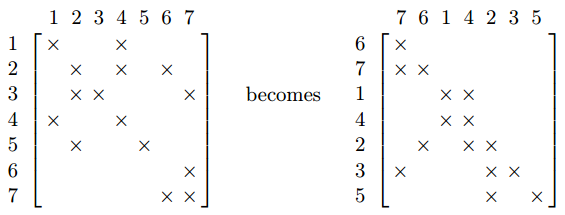
\includegraphics[height=3cm]{png/Singletons.png}
    \caption{Permuting row and column singletons.}
      \label{fig:Singletons}
  \end{figure}
\end{exm}

\begin{rmk}
  In the rest of the section, we consider how $\mathbf{B}_{22}$ can be permuted
  to block triangular form.
\end{rmk}


\begin{defn}
  The algorithm of finding a transversal can be described in either a
  row or a column orientation. We follow the variant that looks at the
  columns one by one and permutes the rows.
  After permutations have been found that place entries in the first
  $k-1$ diagonal positions, we examine column $k$ and seek a row
  permutation that will:
  \begin{enumerate}[(i)]
  \item Preserve the presence of entries in the first $k-1$ diagonal
    positions,
  \item result in column $k$ having an entry in row $k$.
  \end{enumerate}
  The algorithm continues in this fashion extending the transversal by one at
  each stage. Success in this extension is called an
  \emph{assignment}. Sometimes this transversal extension step is
  trivial, which is called a \emph{cheap assignment}.
\end{defn}

\begin{exm}
  In Figure \ref{fig:CheapA}, the assignment in column six is made by
  the interchange of rows six and seven. Figure \ref{fig:NotCheapA}
  shows a simple case where a cheap assignment is not available, but
  the interchange of rows one and seven is adequate the $(1,1)$ entry
  and make a cheap assignment possible in column six.
  \begin{figure}[H]
  \centering
  \subfigure[A cheap assignment for column 6]{
    \label{fig:CheapA}
    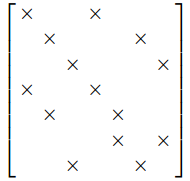
\includegraphics[width=3cm]{png/CheapAssignment.png}
  }
  \hspace{1cm}
  \subfigure[A single preliminary row interchange is needed]{
    \label{fig:NotCheapA}
    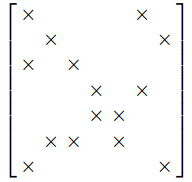
\includegraphics[width=3cm]{png/NotCheapAssignment.png}}
  \caption{Two examples of assignment.}
  \label{fig:Assignment}
\end{figure}
\end{exm}

\begin{defn}
  Sometimes the transversal cannot be extended because the matrix is
  singular for all numerical values of the entries. Such a matrix is
  called \emph{symbolically singular} or \emph{structurally singular}.
\end{defn}

\begin{exm}
  A symbolically singular case is
  $$\left[
    \begin{array}{ccccc}
      \times & \times & & \times & \\
             & & \times & & \times\\
      & & \times & & \times\\
      \times & \times & & \times & \\
      & & \times & & \times\\
    \end{array}
  \right].$$
\end{exm}

\begin{alg}[Transversal extension by depth-first search]
  \label{algo:DFSforTransversal}
  We seek a sequence of columns $c_1,c_2,\ldots,c_j$ with
  $c_1=k$ having entries in rows $r_1,r_2,\ldots,r_j$, with
  $r_i=c_{i+1},\ i=1,2,\ldots,j-1$ and $r_j\geq k.$ Then the sequence of
  row interchanges $(r_1,r_2),\ldots,(r_{j-1},r_j)$ achieves what we
  need. To find this we start with the first entry in column $k$ we take
  its row number to indicate the next column and continue letting the
  first off-diagonal entry in each column indicate the subsequent
  column. In each column, we look for an entry in row $k$ or
  beyond. This sequence has one of the following possible outcomes:
  \begin{enumerate}[(i)]
  \item We find a column with an entry in row $k$ or beyond.
  \item We reach a row already considered.
  \item We come to a dead end (that is a column with no off-diagonal
    entries or one whose off-diagonal entries have all already been considered).
  \end{enumerate}
  In case (i) we have the sequence of columns that we need. In case
  (ii) we take the next entry in the current column. In case (iii), we
  backtrack to the previous column and start again with the next entry there.
\end{alg}

\begin{exm}
  In figure \ref{fig:NotCheapA}, we seek a sequence of
  columns $6,1,7$ by the above algorithm, so the interchange of rows 1
  and 7 is adequate to preserve the $(1,1)$ entry and make a cheap
  assignment possible in column 6. 
\end{exm}

\begin{rmk}
  Always taking the next column rather than trying other rows in the present
column is the depth-first part. Looking to see if there is an entry in 
row k or  beyond is the look-ahead feature.
\end{rmk}
\begin{thm}
  If the matrix order is $n$ and it has $\tau$ entries, the number of elementary
  operations of algorithm~\ref{algo:DFSforTransversal} is at worst proportional to $n\tau$.
\end{thm}

\begin{rmk}
  We assume that a row permutation $\mathbf{P}_1$ has been computed so that
  $\mathbf{P}_\mathbf{1A}$ has entries on every position on its diagonal, then we wish
  to find a permutation matrix $\mathbf{Q}$ such that $\mathbf{Q}^T(\mathbf{P}_1\mathbf{A})\mathbf{Q}$ has the form
  \begin{equation}
    \mathbf{Q^T}(\mathbf{P}_1\mathbf{A})\mathbf{Q}=\left[
    \begin{array}{ccccc}
      \mathbf{B}_{11}& & & & \\
      \mathbf{B}_{21} & \mathbf{B}_{22} & & & \\
      \mathbf{B}_{31} & \mathbf{B}_{32} & \mathbf{B}_{33} & & \\
      \vdots&\vdots&\vdots&\ddots& \\
      \mathbf{B}_{N1}& \mathbf{B}_{N2}& \mathbf{B}_{N3} & \cdots& \mathbf{B}_{NN}\\
    \end{array}
  \right]
  \end{equation}
\end{rmk}

\begin{rmk}
  It is convenient to describe algorithms for this process with the
  help of the directed graphs associated with the matrices. Applying a
  symmetric permutation to the matrix causes no change in the
  associated directed graph except for the relabelling of its nodes.
\end{rmk}

\begin{thm}
  \label{thm:Divide2Part}
  If we cannot find a closed path, we must be able to divide the
  directed graph into two parts such that there is no path from the
  first part to the second. Renumbering the first group of nodes
  $1,2,\ldots,k$ and the seconde group $k+1,\ldots,n$ will produce a
  corresponding matrix in block lower triangular form.
\end{thm}

\begin{defn}
The same process in theorem \ref{thm:Divide2Part} may be applied to
each resulting block until no fuether subdivision is possible. The
sets of nodes corresponding to the resulting diagonal blocks are
called \emph{strong components}.  
\end{defn}

\begin{exm}
  In Figure \ref{fig:SymPermToBTF}, there is no connection from nodes $(1,2)$ to nodes
  $(3,4,5)$. The corresponding matrix is of block lower triangular
  form.
  \begin{figure}[H]
    \centering
    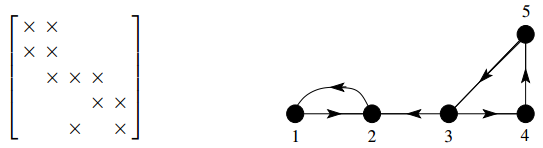
\includegraphics[width=8cm]{png/SymPermToBTF.png}
    \caption{A $5\times 5$ matrix and its digraph(directed graph).}
    \label{fig:SymPermToBTF}
  \end{figure}
\end{exm}

\begin{thm} \label{thm:Sargent}
  If $\mathbf{A}$ is a symmetric permutation of a triangular matrix, there must
  be a node in its digraph from which no path leaves.
\end{thm}

\begin{alg}
  \label{algo:FindingTF}
  The algorithm for finding the triangular form may be built upon the
  theorem \ref{thm:Sargent}:
  \begin{enumerate}
  \item We may start anywhere in the digraph and trace a path until we
    encounter a node from which no paths leave,
  \item number the node at the end of the path first, and remove it
    and all edges pointing to it from the digraph,
  \item continue from the previous node on the path until once again
    we reach a node with no path leaving it.
  \end{enumerate}
\end{alg}

\begin{exm}
  We illustrate the algorithm with the digraph of Figure \ref{fig:DigraphOfSargent}. The
  sequence of paths is illustrated in Figure \ref{fig:AlgorithmOfSargent}.
  \begin{figure}[H]
    \centering
    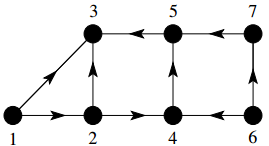
\includegraphics[width=4cm]{png/DigraphToTri.png}
    \caption{A digraph corresponding to a triangular matrix}
    \label{fig:DigraphOfSargent}
  \end{figure}
   \begin{figure}[H]
     \centering
    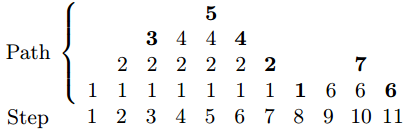
\includegraphics[width=6cm]{png/SequenceOfAlgoSW.png}
    \caption{The sequence of paths used for the Figure
      \ref{fig:DigraphOfSargent} case, where nodes selected for
      ordering are shown in bold.}
     \label{fig:AlgorithmOfSargent}
  \end{figure}
\end{exm}

\begin{defn}
  \emph{A composite node} denotes any group of nodes through which a
  closed path has been found. Edges within a composite node are ignored,
and edges entering or leaving any node of the composite node are regarded as
entering or leaving the composite node. It generalized the idea of
  algorithm~\ref{algo:FindingTF} to the block case.
\end{defn}

\begin{alg}[The algorithm of Sargent and Westerberg]
  
  Starting from any node, a path is followed through the digraph
  until:
  \begin{enumerate}
  \item A closed path is found (identified by encountering the same
    node or composite node tweice), or
  \item a node or composite node is encountered with no edges leaving it.
  \end{enumerate}
  In case (i), all the nodes on the closed path must belong to the same strong
component and the digraph is modified by collapsing all nodes on the closed
path into a single composite node.  The path is now continued from the
composite node.
In case (ii), as for ordinary nodes in the triangular case, the composite node
is numbered next in the relabelling. It and all edges connected to it are removed,
and the path now ends at the previous node or composite node, or starts from
any remaining node if it would otherwise be empty.
\end{alg}

\begin{exm}
   \begin{figure}[H]
    \centering
    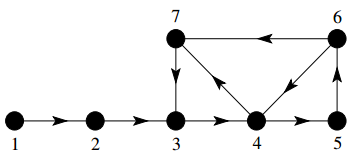
\includegraphics[width=5cm]{png/DigraphToBTri.png}
    \caption{A digraph illustrating the algorithm of Sargent and
      Westerberg.}
    \label{fig:DigraphToBTri}
  \end{figure}
   \begin{figure}[H]
     \centering
    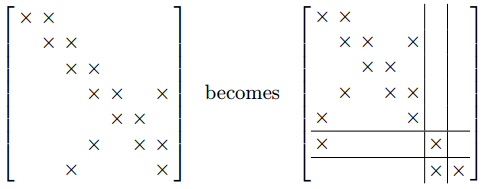
\includegraphics[width=6cm]{png/SequenceOfAlgoSW2.png}
    \caption{The matrices before and after renumbering.}
    \label{fig:MatricesChange}
  \end{figure}
  We illustrate with the example shown in Figure
  \ref{fig:MatricesChange}. Starting the path at node 1, it continues
  $1 \rightarrow 2\rightarrow 3\rightarrow 4\rightarrow 5\rightarrow
  6\rightarrow 4$, then $(4,5,6)$ is recognized as a closed path, and
  nodes 4,5,6 are relabelled as composite node $4'$. The path is
  continued from this composite node to become $1\rightarrow
  2\rightarrow 3\rightarrow 4'\rightarrow 7\rightarrow 3$. Again, a
  closed path has been found and $(3,4',7)$ is labelled as $3'$ and
  the path becomes $1\rightarrow 2\rightarrow 3'.$ Since there are no
  edges leaving $3'$, it is numbered first and removed. The path is
  now $1\rightarrow 2$ and no edges leave node 2, so this is numbered
  second. Finally, node 1 is numbered as the last block. The
  corresponding original and reordered matrices are shown in Figure
  \ref{fig:MatricesChange}.
\end{exm}

\begin{rmk}
  The difficulty with this approach is that there may be large
  overheads associated with the relabelling in the node collapsing
  step. A simple scheme such as labelling each composite node with the
  lowest label of its constituent nodes can result in $\mathcal{O}(n^2)$ relabellings.
\end{rmk}

\begin{exm}
  In Figure successive composite nodes are (4, 5), (3, 4, 5, 6), (2, 3,
  4, 5, 6, 7), (1, 2, 3, 4, 5, 6, 7, 8). In general, such a digraph
  with $n$ nodes will involve $2+4+6+\cdots+n=n^2/4+n/2$ relabellings.
\begin{figure}[H]
  \centering
    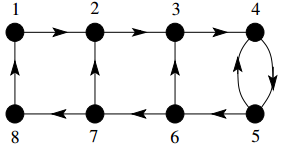
\includegraphics[width=5cm]{png/ManyRelabelling.png}
    \caption{A case causing many relabellings.}
    \label{fig:ManyRelabelling}
  \end{figure}
\end{exm}

\subsection{Local pivotal strategies for sparse matrices}
\label{sec:LocalPivotal}

\begin{defn}
  Suppose Gaussian elimination applied to an $n\times n$ matrix has
  proceeded through the first $k-1$ stages. For each row $i$ in the
  active $(n-k+1)\times(n-k+1)$ submatrix, let $r_i^{(k)}$ denotes the
  number of entries in row $i$. Similarly, let $c_j^{(k)}$ be the
  number of entries in column $j$. Then, the Markowitz criterion is to
  select the entry $a_{ij}^{(k)}$ that minimizes the expression
  \begin{equation}
    \label{eq:MarkowitzCriterion}
    (r_i^{(k)}-1)(c_j^{(k)}-1)
  \end{equation}
  from the entries of the active $(n-k+1)\times(n-k+1)$ submatrix that
  are not too small numerically.
\end{defn}

\begin{rmk}
  An advantage of using \eqref{eq:MarkowitzCriterion} rather than
  $r_i^{(k)}c_j^{(k)}$ is that this forces the algorithm to select a
  row singleton or a column singleton if either is present. Such a
  choice produces no fill-in at all.
\end{rmk}

\begin{thm}
 If $\mathbf{A}$ is symmetric,  the search for the pivot is simplified to
 finding $i$ such that $$r_i^{(k)}=\min\limits_tr_t^{(k)}$$ leading to
 $a_{ii}^{(k)}$ as pivot if $a_{ii}^{(k)}$ is nonzero.
\end{thm}
\begin{rmk}
  It is called the minimum degree algorithm because of its graph
  theoretic interpretation: in the graph assoiated with a symmetric
  sparse matrix, this strategy corresponds to choosing the node for
  the next elimination that has the least edges connected to it.
\end{rmk}

\begin{alg}
  Assoicated with the Markowitz ordering strategy is the need in the
  unsymmetric case to establish a suitable threshold parameter, $u$,
  for numerical stability. In particular, we restrict the Markowitz
  selection to those pivot candidates satisfying the inequality
  \begin{equation}
    \label{eq:MarkowitzThreshold}
    |a_{kk}^{(k)}|\geq u|a_{ik}^{(k)}|,\ i>k,
  \end{equation}
  where $u$ is a preset parameter in the range $0<u\leq 1$.
\end{alg}

\subsection{Ordering sparse mtrices for band solution}
\label{sec:BandSolution}

\begin{rmk}
We consider a different approach to reordering to preserve sparsity,
with algorithms that take a global view of the problem.
\end{rmk}


\begin{defn}
 A sparse matrix in which the nonzero elements are located in a band
 about the main diagonal is called a \emph{band matrix}. If $\mathbf{A}$ is a band matrix, then
 $$a_{ij}=0,\ |i-j|>s \mbox{ for some value } s,$$
 which is illustrated on the left of Figure \ref{fig:bandedMatrix}.
\end{defn}

\begin{defn}
  For a symmetrically structured matirx $\mathbf{A}$ has \emph{bandwidth} $2m+1$ and
  \emph{semibandwidth} $m$ if $m$ is the smallest integer such that
  $a_{ij}=0$ whenever $|i-j|>m.$ For unsymmetric case, we define the
  lower (upper) semibandwidth as the smallest integer $m_l (m_u)$ such
  that if $a_{ij}$ is an entry, $i-j\leq m_l$ ($j-i\leq m_u$). The
  bandwidth is $m_l+m_u+1.$
\end{defn}

\begin{defn}
  $\mathbf{A}$ is of the \emph{variable-band} form (also called skyline form) if
  $$a_{ij}=0,\ j-i>s_i \mbox{ or } a_{ji}=0,\ j-i>t_i$$
  for some values $s_i$ and $t_i,\ i=1,2,\ldots,n$, which is shown on
  the right of Figure \ref{fig:bandedMatrix}.
\end{defn}

\begin{defn}
  When using the variable-band form for a symmetric matrix, we store
  for each row every coefficient between the first entry in the row
  and the diagonal. In the unsymmetric case, we also store for each
  column every coefficient between the first entry in the column and
  the diagonal. The total number of coefficients stored is called the \emph{profile}.
\end{defn}

\begin{figure}[H]
  \centering
    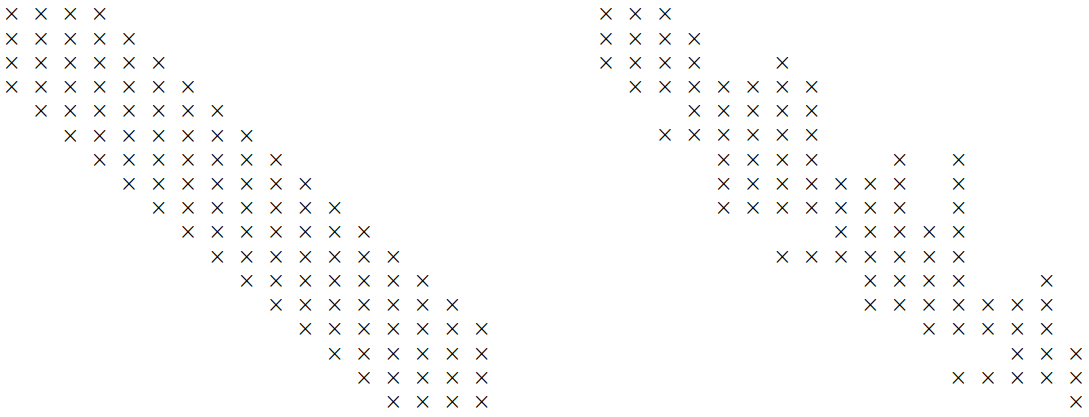
\includegraphics[width=8cm]{png/bandmatrix.png}
    \caption{Band and variable-band matrices.}
    \label{fig:bandedMatrix}
  \end{figure}

  \begin{rmk}
    Finding the banded or variable-band form is based on finding
    permutations to block tridiagonal form. If the blocks are small
    and numerous such a matrix is banded with a small bandwidth.
  \end{rmk}

  \begin{alg}
    The factorization of a block tridiagonal matrix $A$ can be written
    in the form
    $$
    \left[
      \begin{array}{cccccc}
        \mathbf{A}_{11} & \mathbf{A}_{12}& & & & \\
        \mathbf{A}_{21} & \mathbf{A}_{22} & \mathbf{A}_{23} & & &\\
               & \mathbf{A}_{32} & \mathbf{A}_{33} & \cdot & &\\
               & & \cdot & \cdot & \cdot & \\
               & & & \cdot & \cdot & \\
        & & & & \cdot & \mathbf{A}_{NN}
      \end{array}
    \right]=\mathbf{LU},
    $$
    $\mathbf{L}$ and $\mathbf{U}$ can be written in 
    $$
 \mathbf{L}=\left[
      \begin{array}{cccccc}
       \mathbf{I} & & & & & \\
        \mathbf{A}_{21}\mathbf{D}_1^{-1} & \mathbf{I}& & & &\\
               & \ddots & \ddots & & \\
        & &\mathbf{A}_{N,N-1}\mathbf{D}_{N-1}^{-1} & \mathbf{I}
      \end{array}
    \right],
    $$
    $$
    \mathbf{U}=\left[
      \begin{array}{cccccc}
        \mathbf{D}_1 & \mathbf{A}_{12}& & & & \\
         & \mathbf{D}_2& \mathbf{A}_{23}& & &\\
               & & \ddots & \ddots & & \\
               & & & \ddots & \mathbf{A}_{N-1,N} & \\
        & & & & \mathbf{D}_N
      \end{array}
    \right],
    $$
    where
  \begin{align}
    &\mathbf{D}_1=\mathbf{A}_{11},\\
    &\mathbf{D}_i= \mathbf{A}_{ii}-\mathbf{A}_{i,i-1}\mathbf{D}_{i-1}^{-1}\mathbf{A}_{i-1,i},\ i=2,\ldots,N.
  \end{align}
  To use this form to solve a set of equations $\mathbf{Ax=b}$ requires the
  forward substitution steps
  \begin{align}
    &\mathbf{c}_1=\mathbf{b}_1\\
    &\mathbf{c}_i=\mathbf{b}_i-\mathbf{A}_{i,i-1}\mathbf{D}^{-1}_{i-1}\mathbf{c}_{i-1},\ i=2,\ldots,N.
  \end{align}
  followed by the substitution steps
  \begin{align}
   &\mathbf{x}_N=\mathbf{D}^{-1}_N\mathbf{Nc}_N,\\
   &\mathbf{x}_i=\mathbf{D}_i^{-1}\mathbf{c}_i-\mathbf{A}_{i,i+1}\mathbf{c}_{i+1},\ i=N-1,\ldots,1.
  \end{align}
\end{alg} 

\begin{rmk}
   We hope to find an automatic ordering algorithm, such algorithms
   for the symmetric case are the subject of next section.
 \end{rmk}
 
\begin{alg}[Cuthill-McKee algorithm]
  Symmetric permutations of a symmetric matrix correspond to
  relabellings of the nodes of the associated graph and it is easier
  to describe algorithms in terms of relabelling graphs.
  The following is the steps of Cuthill-McKee algorithm:
  \begin{enumerate}[(i)]
  \item Divide the nodes into \emph{level sets}, $S_i$, with
  $S_1$ consisting of a single node. The next, $S_2$, consists of all
  the neighbours of this node. The set $S_3$ consists of all the
  neighbours of the nodes in $S_2$ that are not in $S_1$ or $S_2$. The
  general set $S_i$ consists of lal the neighbours of the nods of
  $S_{i-1}$ that are not in $S_{i-2}$ and $S_{i-1}$.
\item Order within each block $S_i$ by taking first those nodes that
  are neighbours of the first node in $S_{i-1}$, then those that are
  neighbours of the second node in $S_{i-1}$, and so on.
  \end{enumerate}
\end{alg}

\begin{exm}
  The ordering of the Figure \ref{fig:CMcase} could have come from
  level sets (1), (2-4), (5-7), (8-10), (11-13), (14-16), (17) and the
  corresponding matrix shown in Figure \ref{fig:CMcaseMatrix}, is
  block tridiagonal with diagonal blocks having orders 1, 3, 3, 3, 3, 3
  and 1.

  \begin{figure}[H]
    \centering
    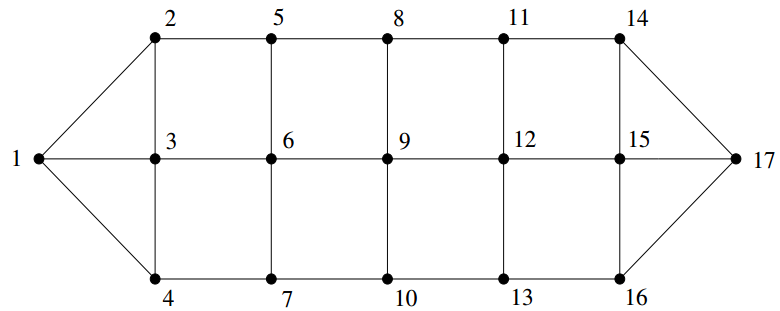
\includegraphics[width=8cm]{png/CMcase.png}
    \caption{A graph with an obviously good node order.}
    \label{fig:CMcase}
  \end{figure}
  \begin{figure}[H]
    \centering
    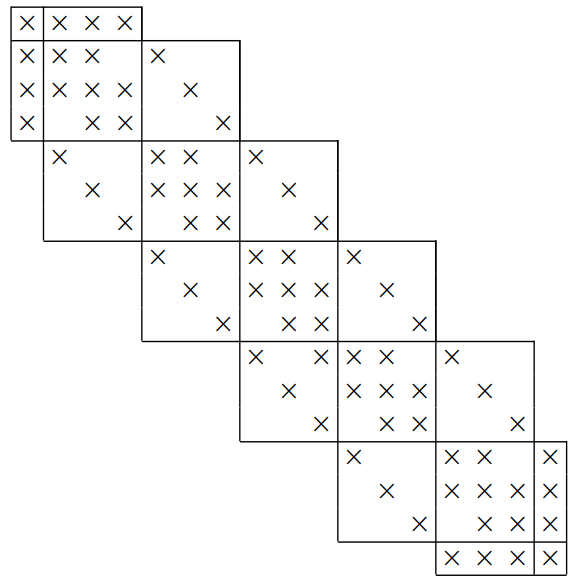
\includegraphics[width=6cm]{png/CMcaseMatrix.png}
    \caption{The matrix corresponding to the Figure \ref{fig:CMcase}
      graph.}
    \label{fig:CMcaseMatrix}
  \end{figure}
\end{exm}

\begin{alg}[the Reverse Cuthill-McKee algorithm(RCM)]
 The only difference with the Cuthill-McKee algorithm is that the
 reverse Cuthill-McKee algorithm orders from the last level set to $S_1$.  
\end{alg}

\begin{rmk}
  Reversing the Cuthill-McKee order often yields a  worthwhile
  improvement, not in the bandwidth, but in the total storage required
  within the variable-band form (the profile) and in the number of
  arithmetic operations required for variable-band factorization. 
\end{rmk}

\begin{exm}
  the Cuthill-McKee order (with level sets (1), (2), (3-7)) is shown
  in Figure \ref{fig:CMorder} and there are 20 zeros within the
  variable-band form. On reversing the order (Figure
  \ref{fig:RCMorder}) all these zeros move outside the form and will
  not need storage. 

  \begin{figure}[H]
    \centering
    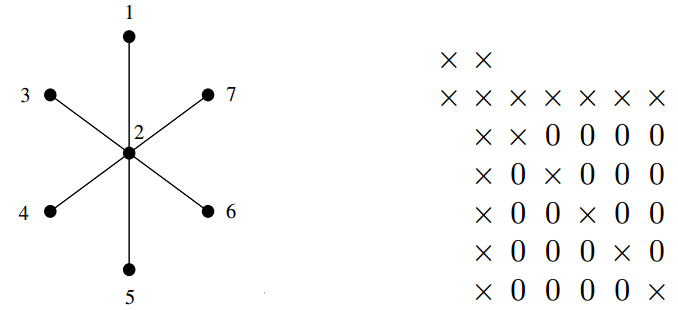
\includegraphics[width=8cm]{png/CMorder.png}
    \caption{A graph and its associated matrix, ordered by Cuthill-McKee.}
    \label{fig:CMorder}
  \end{figure}

  \begin{figure}[H]
    \centering
    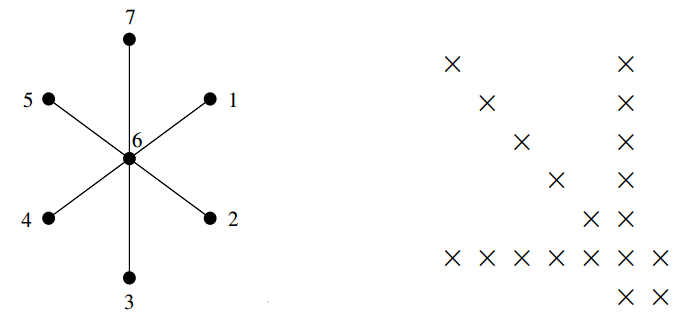
\includegraphics[width=8cm]{png/RCMorder.png}
    \caption{As Figure~\ref{fig:CMorder}, but with order reversed.}
    \label{fig:RCMorder}
  \end{figure}
\end{exm}

\begin{alg}[choosing the starting node for RCM algorithm]
  Each variable in the final level set $S_k$ should be tried as a
  starting node. If one of these nodes produces more than $k$ level
  sets, then this variable replaces the starting node and the new
  level sets are examined, continuing in this way until no further
  increase in the number of level sets is obtained.
\end{alg}

\begin{rmk}
  There are two limitations of the methods of this section:
  \begin{enumerate}
  \item They tend to be less effective when the problems are fully
    two-dimensional, exemplified by a large square grid.
  \item The banded methods are the fundamental sequential nature of
    these orderings. Each computation in the factorization and the
    solve comes from the previous computation. Thus, the methods tend
    to do poorly in a parallel environment.
  \end{enumerate} 
\end{rmk}

\subsection{Orderings based on dissection}
\label{sec:Dissection}

\begin{defn}
  There are two desirable form: \emph{bordered block diagonal form} and
  \emph{doubly-bordered block diagonal form}, which are illustrated in Figure \ref{fig:BBTF}
  and Figure \ref{fig:DBBTF}.

  \begin{figure}[H]
    \centering
    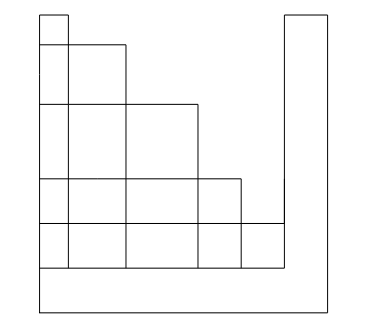
\includegraphics[width=4cm]{png/BorderedBlockDF.png}
    \caption{Bordered block triangular form.}
    \label{fig:BBTF}
  \end{figure}
  \begin{figure}[H]
    \centering
    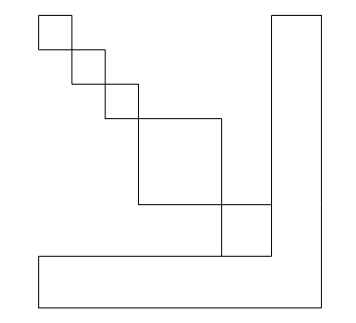
\includegraphics[width=4cm]{png/DBorderedBlockDF.png}
    \caption{Doubly-bordered block triangular form.}
    \label{fig:DBBTF}
  \end{figure}
  
\end{defn}
\begin{exm}
  To establish the basic idea, consider the graph in Figure
  \ref{fig:onewayDissectionCase} with the
  columns in the order $(1,2,4,5,7,8,10,11,3,6,9).$ A way to motivate
  this ordering is to look at the entire graph, and select nodes
  which, when removed, dissect the graph into smaller pieces. The
  effect of this ordering can be seen in the matrix pattern in
  Figure \ref{fig:onewayDissectionCaseMatrix}. We make two observations about this matrix pattern:
  \begin{enumerate}
  \item The ordering leads to a matrix that has a bordered block diagonal
form with four diagonal blocks. Fill-in is confined to the diagonal
blocks and the borders.
\item Factorization of the first four diagonal blocks can be performed independently,
allowing an easy exploitation of parallelism.
\end{enumerate}

\begin{figure}[H]
  \centering
  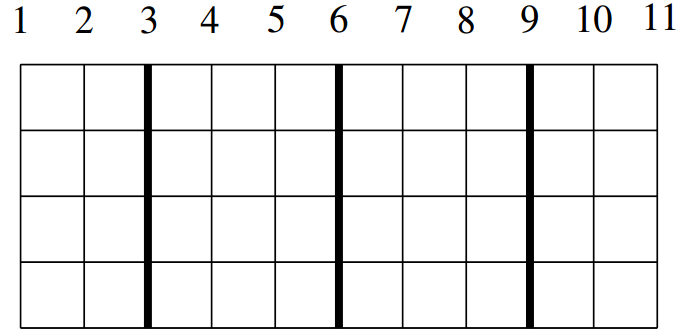
\includegraphics[width=7cm]{png/onewayDissectionCase.png}
  \caption{A regular $5\times 11$ grid problem, one-way dissected.}
  \label{fig:onewayDissectionCase}
\end{figure}
\begin{figure}[H]
  \centering
  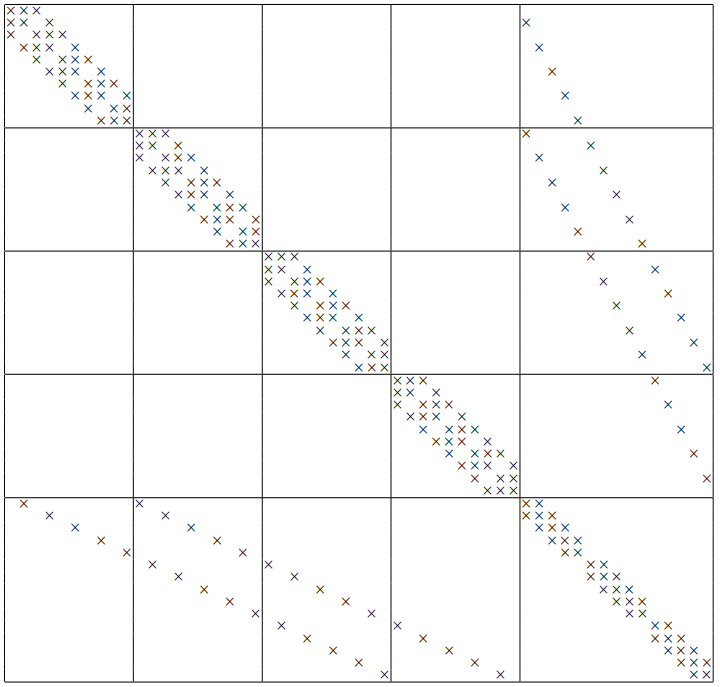
\includegraphics[width=8cm]{png/onewayDissectionMatrix.png}
  \caption{The matrix arising from one-way dissection of the problem
    in Figure \ref{fig:onewayDissectionCase}.}
  \label{fig:onewayDissectionCaseMatrix}
\end{figure}
\end{exm}

\begin{alg}
  Similarly to the way we dealt with the block tridiagonal forms in
  Section \ref{sec:BandSolution}, The factorization of a
  doubly-bordered block tridiagonal matrix $\mathbf{A}$ can be written
    in the form
    $$
    \left[
      \begin{array}{ccccc}
        \mathbf{A}_{11} & & & & \mathbf{A}_{1N} \\
        & \mathbf{A}_{22} & & & \mathbf{A}_{2N}\\
               & & \mathbf{A}_{33} & & \mathbf{A}_{3N}\\
            &   & & \ddots & \vdots  \\
        \mathbf{A}_{N1}& \mathbf{A}_{N2}& \mathbf{A}_{N3}& \cdots & \mathbf{A}_{NN}
      \end{array}
    \right]=\mathbf{LU},
    $$
    $\mathbf{L}$ and $\mathbf{U}$ can be written in 
    $$
 \mathbf{L}=\left[
      \begin{array}{ccccc}
        \mathbf{I} & & & &  \\
        & \mathbf{I}& & & \\
               & & \mathbf{I}& & \\
               & & & \ddots&  \\
        \mathbf{A}_{N1}\mathbf{D}_1^{-1}& \mathbf{A}_{N2}\mathbf{D}_2^{-1}& \mathbf{A}_{N3}\mathbf{D}_3^{-1}& \cdots & \mathbf{I}
      \end{array}
    \right],
    $$
    $$
    \mathbf{U}=\left[
      \begin{array}{ccccc}
        \mathbf{D}_1 & & & & \mathbf{A}_{1N} \\
         & \mathbf{D}_2& & & \mathbf{A}_{2N}\\
               & & \mathbf{D}_3& & \mathbf{A}_{3N}\\
               & & & \ddots& \vdots \\
        & & & & \mathbf{D}_N
      \end{array}
    \right],
    $$
    where
  \begin{align}
    &\mathbf{D}_i=\mathbf{A}_{ii},\ i=1,2,\ldots,N-1.\\
    &\mathbf{D}_N= \mathbf{A}_{NN}-\sum\limits_{j=1}^{N-1}\mathbf{A}_{Nj}\mathbf{D}_{j}^{-1}\mathbf{A}_{jN}.
  \end{align}
  To use this form to solve a set of equations $\mathbf{Ax=b}$ , we can carry
  out the solution in the following way:
  \begin{align}
    &\mathbf{c}_i=\mathbf{b}_i,\ i=1,2,\ldots,N-1\\
    &\mathbf{c}_N=\mathbf{b}_N-\sum\limits_{j=1}^{N-1}\mathbf{A}_{Nj}\mathbf{D}^{-1}_{j}\mathbf{c}_{j},
  \end{align}
  followed by the substitution steps
  \begin{align}
   &\mathbf{x}_N=\mathbf{D}^{-1}_N\mathbf{c}_N,\\
   &\mathbf{x}_i=\mathbf{D}_i^{-1}(\mathbf{c}_i-\mathbf{A}_{iN}\mathbf{c}_{N}),\ i=N-1,\ldots,1.
  \end{align}
\end{alg}

\begin{alg}[Finding the dissection cuts for one-way dissection]
  For automatic one-way dissection of a general problem, George (1980)
  proposed the algorithm for finding the dissection cuts:
  \begin{enumerate}[(i)]
  \item  Firstly, generate a good level structure, as in Section \ref{sec:BandSolution}.
  \item Compute the average number of nods at each level, say $m$.
  \item Take points from each of the level sets $S_j$ where
    \begin{equation}
      \label{eq:DissectionCutsLevelSet}
      j=\lfloor i\delta+0.5\rfloor,\ i=1,2,\ldots
    \end{equation}with spacing
    \begin{equation}
      \label{eq:DissectionCutsSpacing}
      \delta=\sqrt{\frac{3m+13}{2}}.
    \end{equation}
  \end{enumerate}
  The formula \eqref{eq:DissectionCutsSpacing} for the spacing was
  chosen by George on the basis of numerical experiments and analysis
  of regular grids, with the aim of keeping storage requirements
  low. It would suffice to place all the points in the level sets
  \eqref{eq:DissectionCutsLevelSet} in the last block and the points
  in the intervening groups of level sets into the other blocks.
\end{alg}

\begin{defn}
  The \emph{row graph} of a matrix $A$ is the graph with vertices that
  correspond to the rows of $A$ and with an edge between two vertices
  if and only if there is at least one column that has an entry in
  both of the corresponding rows.
\end{defn}

\begin{exm}
  There is an example of a matrix and its row graph in Figure \ref{fig:RowGraph}.
  \begin{figure}[H]
    \centering
    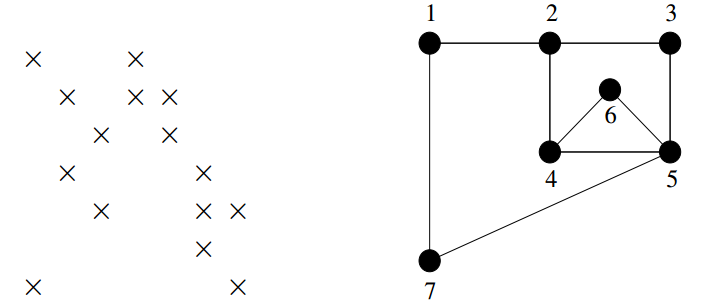
\includegraphics[width=7cm]{png/RowGraph.png}
    \caption{A matrix and its associated row graph.}
    \label{fig:RowGraph}
  \end{figure}
\end{exm}
 
\begin{prop}
  The graph of $\mathbf{AA^T}$ is the row graph of $\mathbf{A}$.
\end{prop}

\begin{defn}
  A \emph{hypergraph} is a generalization of a graph in which an edge can
  join any number of vertices. The generalized edges are called
  \emph{nets} (also known as \emph{hyperedges}). The vertices in a net
  are called its \emph{pins} and \emph{the size of a net} is its
  number of pins. \emph{The degree of a vertex} is the number of nets in
  which it is a pin. Vertex $i$ can have an associated \emph{weight} $w_i$
  and net $i$ can have an associated \emph{cost} $c_i$.
\end{defn}

\begin{defn}
  In a partition, the set of vertices (rows) is divided into $k$
  distinct non-empty \emph{parts} and a net (column) is regarded as being
  \emph{connected} to a part if it has at least one pin in the part.
\end{defn}

\begin{thm}
  By permuting the vertices so that those in each part are together
  and permuting the nets so that those with pins only in part 1 come
  first, then those with pins only in part 2, and then those with pins
  only in part $k$, and finally those with pins in more than one part,
  we obtain the singly bordered block diagonal form illustrated in
  Figure \ref{fig:SinglyBBDF}. 
  \begin{figure}[H]
    \centering
    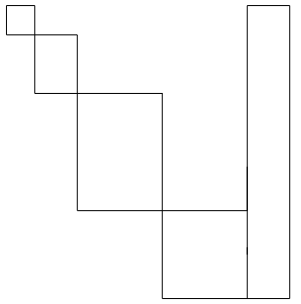
\includegraphics[width=4cm]{png/SinglyBBDF.png}
    \caption{A singly bordered block diagonal form.}
    \label{fig:SinglyBBDF}
  \end{figure}
\end{thm}

\begin{defn}
  The \emph{connectivity} of net (column) $i$, denoted by $\lambda_i$,
  is defined as the number of parts to which it is connected. It is
  said to be \emph{cut} (or \emph{external}) if $\lambda_i>1$. It is the cut nets
  that we permute to the border.
\end{defn}

\begin{defn}
  A partition has an associated \emph{cost}. The two most common are
  the sum of the costs $c_i$ of the cut nets and the sum of the
  weighted sums $c_i(\lambda_i-1)$ of the cut nets. 
\end{defn}

\begin{prop}
  With $c_i=1$, the first cost is the number of columns in the border
  and the second cost corresponds to the amount of communication for
  distributed matrix-vector multiplication.
\end{prop}

\begin{rmk}
  As in the case of graphs, a good partitioning should minimize the
  cost while maintaining a balance between the parts. If the weight
  $W_i$ of part $i$ is defined as the sum of the weights $w_i$ of the
  vertices (rows) in it, a common \emph{balance criterion} is to
  require
  \begin{equation}
    \label{eq:BalanceCriterion}
    W_i\leq W_{avg}(1+e),\ \forall i=1,\ldots,k
  \end{equation}
  where $W_{avg}$ is the average weight of a part and $e$ is a
  tolerance on balance, typically between 0.25 and 1.0.
\end{rmk}

\begin{rmk}
  We seek to partition the rows into two sets such that only a few
  columns have entries in both sets.
\end{rmk}

\begin{defn}
  The \emph{net-cut} is defined as the number of columns with entries
  in both partitions and will be equal to the number of border columns
  in the reordered form.
\end{defn}

\begin{defn}
  A \emph{boundry row} is a row in one set of the current partition
  that is connected in the row graph to a row in the other set of the
  partition (has an entry in the same column as a row of the other
  partition).
\end{defn}

\begin{defn}
  For each row, we can compute the change in the net-cut value caused
  if the row were moved to the other partition. This is called the \emph{gain}.
\end{defn}

\begin{alg}
  The algorithm is used to improve a given partition:
\begin{figure}[H]
    \centering
    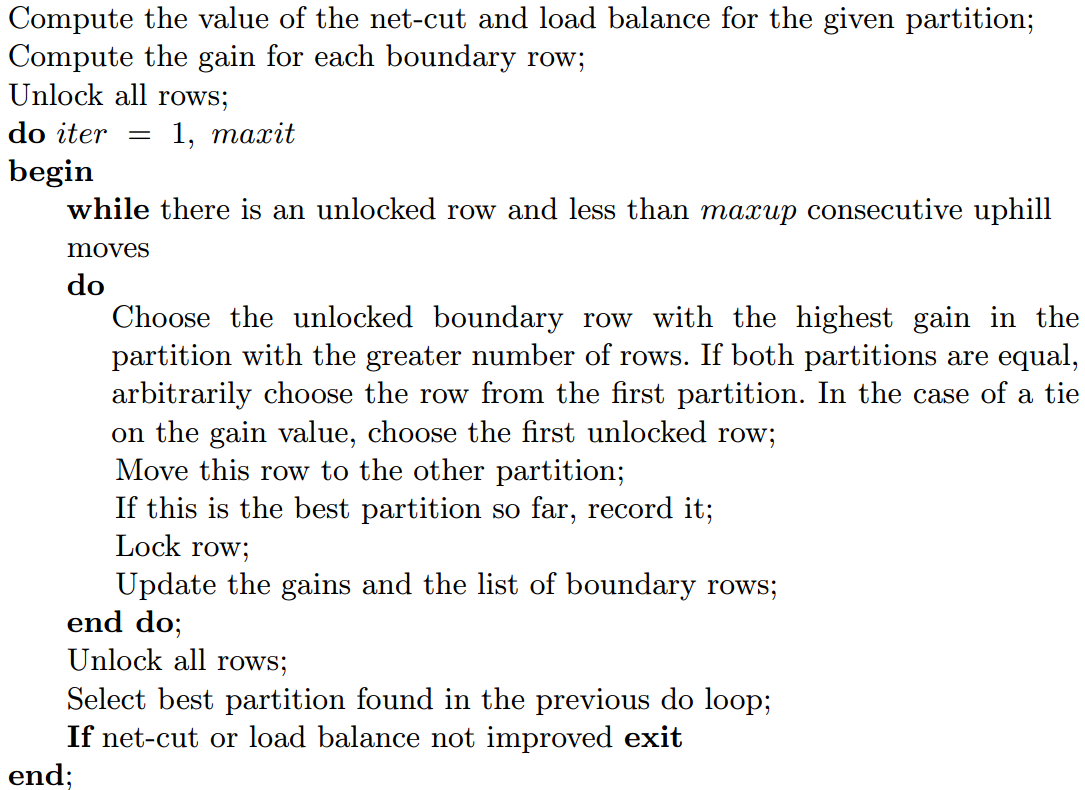
\includegraphics[width=9cm]{png/LinAlgorithm.png}
    \caption{A summary of the Kernighan and Lin (1970) algorithm in
      pseudo-algol.}
    \label{fig:LinAlgorithm}
  \end{figure}
\end{alg}

\begin{rmk}
  To find an appropriate starting point for the Kernighan and Lin
  algorithm, we would use this algorithm wihin a multilevel
  scheme. The strategy is coarsening algorithm to coarsen the matrix recursively
  and then applies the Kernighan and Lin algorithm to the graph of
  each level.
\end{rmk}

\begin{alg}
  The strategy used by \texttt{MONET} algorithm for coarsening the pattern of
  the unsymmetric matrix is to recognize and combine pairs of rows
  that have similar patterns. The algorithm for doing this is given in
  Figure \ref{fig:Monet}. 

  \begin{figure}[H]
    \centering
    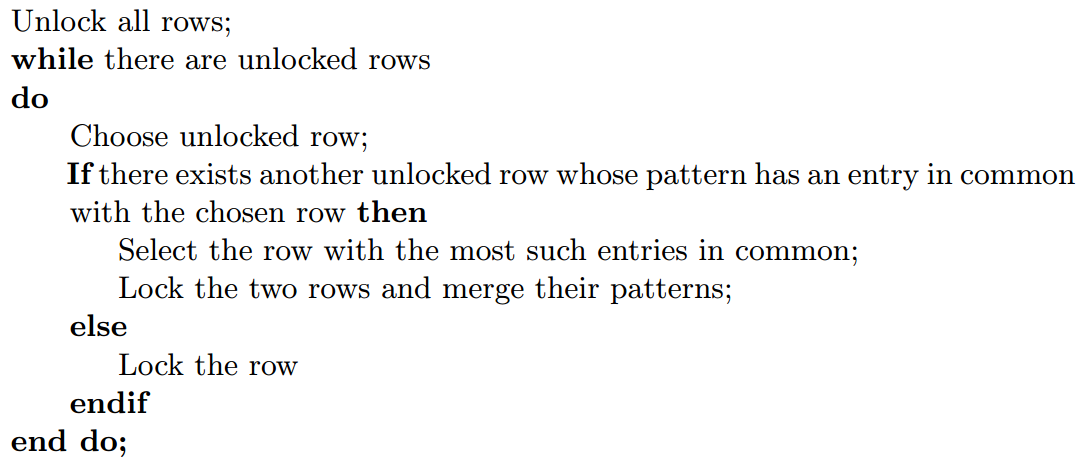
\includegraphics[width=9cm]{png/MONET.png}
    \caption{A summary of the \texttt{MONET} coarsening algorithm in
      pseudo-algol.}
    \label{fig:Monet}
  \end{figure}

  This coarsening is continued until the number of rows in the coarse matrix is
less than a preset number (default 100 in \texttt{HSL\_MC66}) or the ratio of the number
of rows in consecutive matrices is more than a preset fraction (default 0.75 in
\texttt{HSL\_MC66}).
\end{alg}

\begin{rmk}
  The \texttt{MONET} approach coarsens the matrix recursively and then applies
the Kernighan and Lin algorithm to the graph
corresponding to the coarsest matrix from an arbitrary starting partition with
roughly equal numbers of rows in its two sets and with its parameters set very
high in the hope of getting a near optimal partition on this small
matrix.

This partition is then prolongated to the next finer graph through expanding the
rows that were collapsed in that level of the coarsening. The Kernighan and Lin
algorithm is then applied with this partition as the starting point
and the process is repeated up to the finest graph corresponding to the original
matrix. The columns of the net-cut are moved to the border.
\end{rmk}
%%% Local Variables:
%%% mode: latex 
%%% TeX-master: "LU_MathDocument"
%%% End:
